\RequirePackage{fix-cm}
%
\RequirePackage{amsmath}

%\documentclass{svjour3}                     % onecolumn (standard format)
%\documentclass[smallcondensed]{svjour3}     % onecolumn (ditto)
%\documentclass[smallextended]{svjour3}       % onecolumn (second format)
% \documentclass[twocolumn]{svjour3}          % twocolumn
%\documentclass[letterpaper, 12pt, twocolumn]{article}
\documentclass{article}
\usepackage[cm]{fullpage}
%\usepackage[margin=1in]{geometry}
\usepackage{amssymb}
\usepackage{graphicx}
\usepackage[utf8]{inputenc}
\usepackage{indentfirst}
%\usepackage{physics}
\newcommand{\me}{\mathrm{e}}
\usepackage{amsmath}

%\usepackage[round]{natbib}
%\usepackage{apacite}
\usepackage{url}

% For the flow charts
\usepackage{tikz}
\usetikzlibrary{external}
\tikzexternalize

\usetikzlibrary{shapes.geometric, arrows, calc, positioning}
\tikzstyle{startstop} = [rectangle, thick, rounded corners=2.5mm, minimum width=2cm, minimum height=5mm,text centered, draw=black]
\tikzstyle{io} = [trapezium, thick, trapezium left angle=70, trapezium right angle=110, text width=3.75cm, minimum height=0.5cm, text centered, draw=black]
\tikzstyle{process} = [rectangle, thick, minimum width=2.5cm, text width=4cm, minimum height=0.5cm, text centered, draw=black]
\tikzstyle{decision} = [diamond, thick, minimum width=3cm, minimum height=1cm, text centered, draw=black]
\tikzstyle{dottedbox} = [rectangle, dotted, thick, minimum width=2.5cm, text width=2.8cm, minimum height=0.5cm, text centered, draw=black]
\tikzstyle{arrow} = [thick,->,>=stealth]
\tikzstyle{dottedarrow} = [thick, dotted,->,>=stealth]



\usepackage{pgfplots}
\usepgfplotslibrary{patchplots}
\pgfplotsset{compat=newest, samples=065} %Set this value to 65 for the final version
%\usepgfplotslibrary{dateplot} 


%\providecommand{\keywords}[1]{\textbf{\textit{Index terms---}} #1}

%\journalname{Journal of Science Education and Technology}

\begin{document}


\title{Algorithm to generate multi-factorial experiments to teach experimental design%\thanks{Grants or other notes
%about the article that should go on the front page should be
%placed here. General acknowledgments should be placed at the end of the article.}
}
%\subtitle{Do you have a subtitle?\\ If so, write it here}
%\titlerunning{Short form of title}        % if too long for running head
\author{A.C.~Delgado-Chavez  \and
        N.~Balagurusamy \and
        R.~Narayanasamy \and
        S.~K.~Gadi
}
%\authorrunning{Short form of author list} % if too long for running head
% The correct dates will be entered by the editor
\begin{figure}
	\centering
	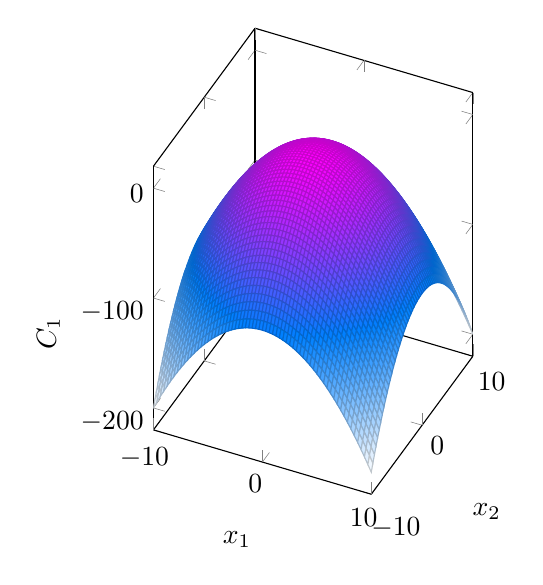
\begin{tikzpicture}
		\begin{axis}[
			width=0.465\textwidth,	
			height = 7.5cm,
			colormap/cool,
			xlabel=$x_1$,
			ylabel=$x_2$,
			zlabel=$C_1$,
			]
			\addplot3[
			surf,
			%samples=10,
			domain=-10:10,
			]
			{-x^2-y^2};
			%\addlegendentry{$\frac{sin(r)}{r}$}
		\end{axis}
	\end{tikzpicture}
	\caption{Quadratic concave function $C_1(x_1, x_2)$.}
	\label{Fig:TwoVariablePolynomial}
\end{figure}



\begin{figure}
	\centering
	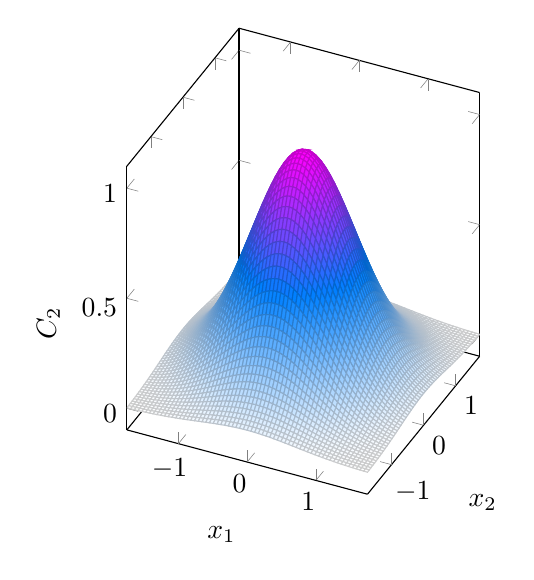
\begin{tikzpicture}
	\begin{axis}[
		width=0.50\textwidth,	
		height = 7.5cm,
		colormap/cool,
		xlabel=$x_1$,
		ylabel=$x_2$,
		zlabel=$C_2$,
		]
		\addplot3[
		surf,
		%samples = 10,
		domain=-1.75:1.75,
		]
		{exp(-x^2-y^2)};
	\end{axis}
	\end{tikzpicture}
	\caption{Two variable Gaussian function $C_2(x_1, x_2)$.}
	\label{Fig:TwoVarGaussian}
\end{figure}



\begin{figure}
	\centering
	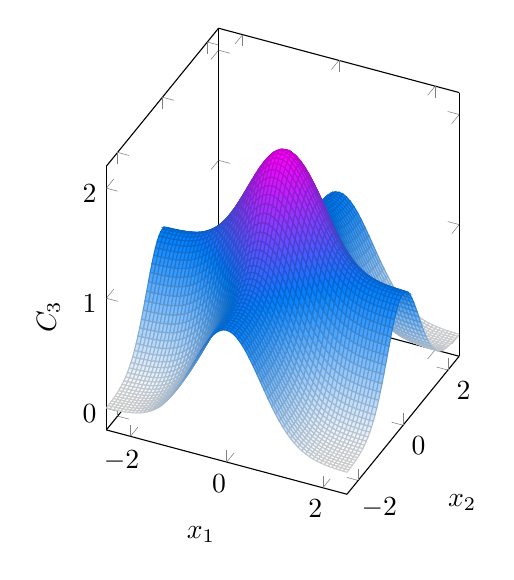
\begin{tikzpicture}
	\begin{axis}[
		width=0.50\textwidth,	
		height = 7.5cm,
		colormap/cool,
		xlabel=$x_1$,
		ylabel=$x_2$,
		zlabel=$C_3$,
		]
		\addplot3[
		surf,
		%samples = 50,
		domain=-2.5:2.5,
		]
		{exp(-x^2)+exp(-y^2)};
	\end{axis}
	\end{tikzpicture}	
	\caption{Modified version of Gaussian function $C_3(x_1, x_2)$.}
	\label{Fig:2GussianFunctionModified}
\end{figure}



\begin{figure}
	\centering
	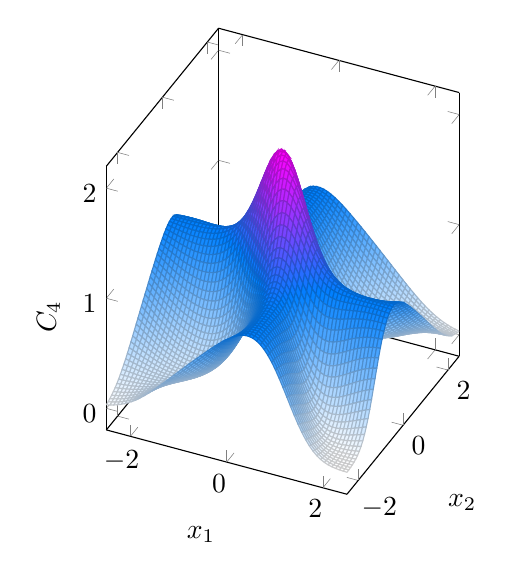
\begin{tikzpicture}
	\begin{axis}[
		width=0.50\textwidth,	
		height = 7.5cm,
		colormap/cool,
		xlabel=$x_1$,
		ylabel=$x_2$,
		zlabel=$C_4$,
		]
		\addplot3[
		surf,
		%samples = 50,
		domain=-2.5:2.5,
		]
		{exp(-(x+0.49*sin(deg(x+y)))^2)+exp(-(y+0.49*sin(deg(x+y)))^2)};
	\end{axis}
	\end{tikzpicture}
	\caption{The proposed function $C_4(x_1, x_2)$ for $a = 0.49$.}
	\label{Fig:TwoVarNovelFunc}
\end{figure}

\begin{figure}
	\centering
	\begin{tikzpicture}
	\begin{axis}[
	width=0.50\textwidth,	
	height = 7.5cm,
	colormap/cool,
	xlabel=$x_1$,
	ylabel=$x_2$,
	zlabel=$C_4$,
	]
	\addplot3[
	surf,
	%samples = 50,
	domain=-3:3	,
	]
	%{exp(-(x+2*sin(deg(x+y)))^2) + exp(-(y+2*sin(deg(x+y)))^2)};
	%{exp(-(x + .49*sin((40.1415*6/6*(x + y))))^2) + exp(-(y + .49*sin((40.1415*6/6*(x + y))))^2)};
	{exp(-(x+exp(1*(x^2+y^2)))^2) + exp(-(y+exp((x^2+y^2)*1))^2)};
	\end{axis}
	\end{tikzpicture}
	\caption{The proposed-- function $C_4(x_1, x_2)$ for $a = 0.49$.}
	\label{Fig:TwoVarNovelFunc3}
\end{figure}
\section{adf}

\pagebreak
\begin{figure}
	\centering
	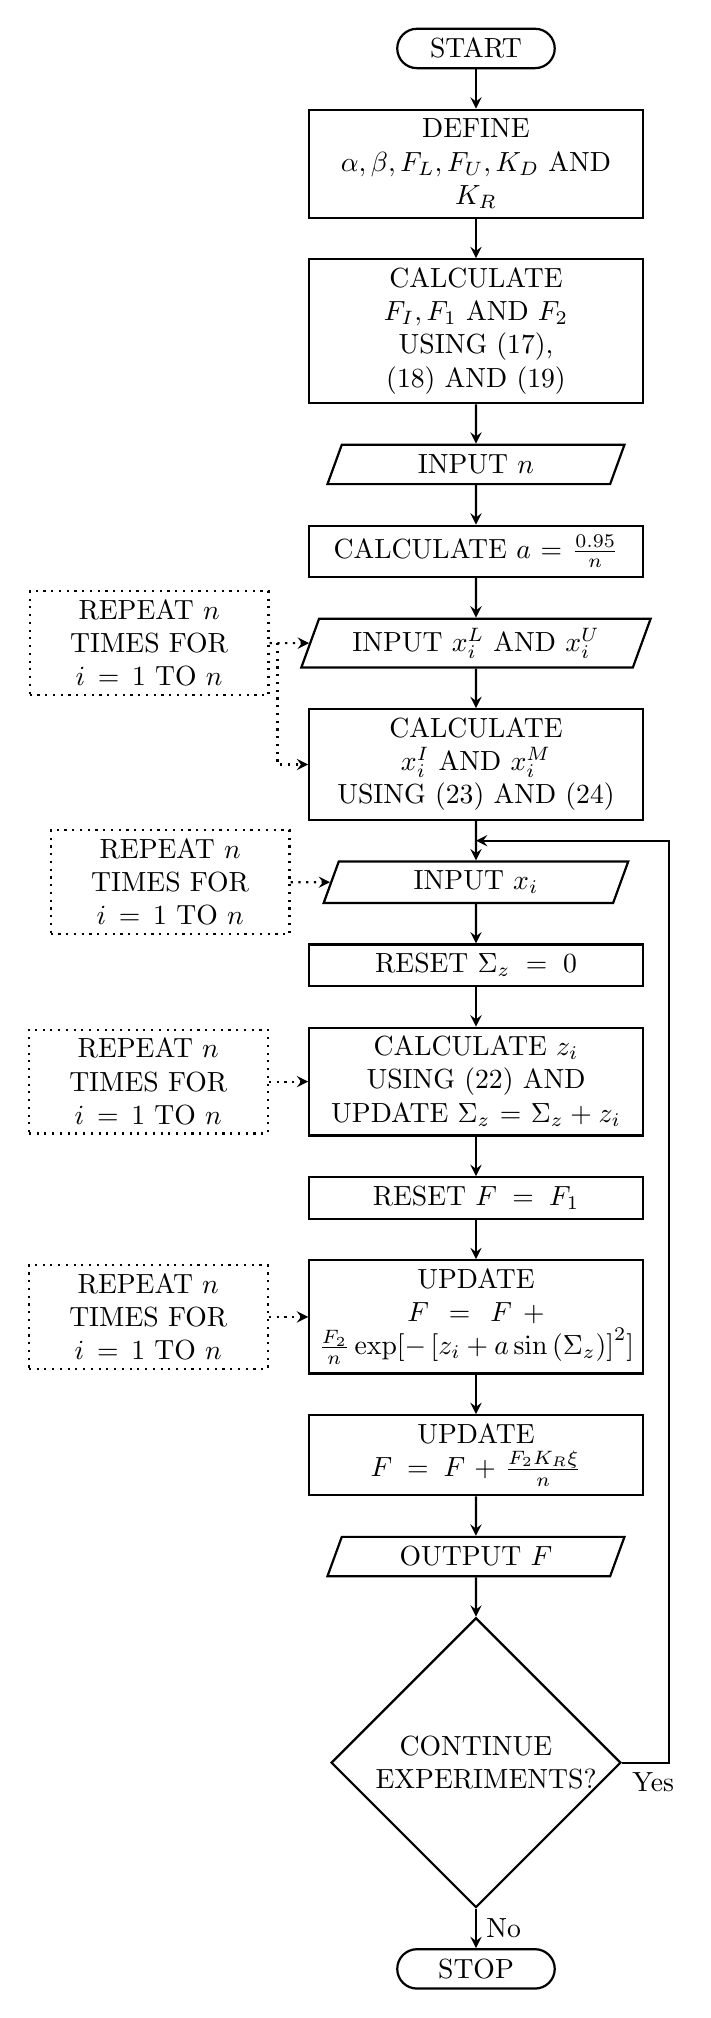
\begin{tikzpicture}[node distance = 5mm, auto]
		\node (Start) [startstop] {START};
		\node (Define) [process, below = of Start] {DEFINE $\alpha, \beta, F_L, F_U, K_D$~AND $K_R$};
		\node (Calculate01) [process, below =of Define] {CALCULATE\\$F_I, F_1$ AND $F_2$\\USING (17), (18) AND (19)};
		\node (Input01) [io, below = of Calculate01, text width=3cm] {INPUT $n$};
		\node (Calculate01a) [process, below = of Input01] {CALCULATE $a=\frac{0.95}{n}$};
		\node (Input02) [io, below = of Calculate01a] {INPUT $x_i^L$~AND~$x_i^U$};
		\node (Calculate02) [process, below = of Input02] {CALCULATE\\$x_i^I$ AND $x_i^M$\\USING (23) AND (24)};
		\node (Input03) [io, below = of Calculate02, text width=3.25cm] {INPUT $x_i$};
		\node (Calculate03) [process, below = of Input03] {RESET $\Sigma_z=0$};
		\node (Calculate04) [process, below = of Calculate03] {CALCULATE $z_i$\\ USING (22) AND\\UPDATE $\Sigma_z = \Sigma_z + z_i$};
		\node (Calculate05) [process, below = of Calculate04] {RESET $F=F_1$};
		\node (Calculate06) [process, below = of Calculate05] {UPDATE\\  $F=F+\frac{F_2}{n} \exp[-\left[z_i + a\sin\left(\Sigma_z\right)\right]^2]$};
		\node (Calculate07) [process, below = of Calculate06] {UPDATE	\\ $F=F+\frac{F_2K_R\xi}{n}$};
		\node (Output03) [io, below = of Calculate07, text width=3cm] {OUTPUT $F$};
		\node (Decision01) [decision, below = of Output03, text width=2.55cm] {CONTINUE\\EXPERIMENTS?};
		\node (Stop) [startstop, below = of Decision01] {STOP};

		\node (ForBox01) [dottedbox, left = of Input02, left = 5mm] {REPEAT $n$ TIMES FOR $i=1$ TO $n$};
		%\node (ForBox02) [dottedbox, left of=Calculate02, left = 2.25cm] {REPEAT $n$ TIMES FOR $i=1$ TO $n$};
		\node (ForBox03) [dottedbox, left = of Input03, left = 5mm] {REPEAT $n$ TIMES FOR $i=1$ TO $n$};
		\node (ForBox04) [dottedbox, left = of Calculate04, left = 5mm] {REPEAT $n$ TIMES FOR $i=1$ TO $n$};
		\node (ForBox05) [dottedbox, left = of Calculate06, left = 5mm] {REPEAT $n$ TIMES FOR $i=1$ TO $n$};

 		%\node (stop) [startstop, below of=calculate1, below = 0mm] {STOP};
		\draw [arrow] (Start) -- (Define);
		\draw [arrow] (Define) -- (Calculate01);
		\draw [arrow] (Calculate01) -- (Input01);
		\draw [arrow] (Input01) -- (Calculate01a);
		\draw [arrow] (Calculate01a) -- (Input02);
		\draw [arrow] (Input02) -- (Calculate02);
		\draw [arrow] (Calculate02) -- (Input03);
		\draw [arrow] (Input03) -- (Calculate03);
		\draw [arrow] (Calculate03) -- (Calculate04);
		\draw [arrow] (Calculate04) -- (Calculate05);
		\draw [arrow] (Calculate05) -- (Calculate06);
		\draw [arrow] (Calculate06) -- (Calculate07);
		\draw [arrow] (Calculate07) -- (Output03);
		\draw [arrow] (Output03) -- (Decision01);
		\draw [arrow] (Decision01) -- node[anchor=west]{No}(Stop);
		\draw [arrow] ($ (Decision01.east) $)node[anchor=north west]{Yes}  -- ++(0.6,0.00) |- ($ (Input03.north) + (0mm,2.5mm) $);

		\draw [dottedarrow] (ForBox01) -- (Input02);
		%\draw [dottedarrow] (ForBox02) -- (Calculate02);
		\draw [dottedarrow] ($(ForBox01.east) + (1mm,0mm)$) |- (Calculate02);
		\draw [dottedarrow] (ForBox03) -- (Input03);
		\draw [dottedarrow] (ForBox04) -- (Calculate04);
		\draw [dottedarrow] (ForBox05) -- (Calculate06);
	\end{tikzpicture}
	\caption{Flowchart of the proposed algorithm}
	\label{Fig:AlgorithmInFlowchart}
\end{figure}




\begin{figure}
	\centering
	\begin{tikzpicture}
	\begin{axis}
		[
		width=0.50\textwidth,	
		xlabel=$x_1$,
		ylabel=$x_2$,
		zlabel=$C$,
		view={0}{90}
		]
		\addplot3[contour gnuplot ={number=20,
			labels=false,
		},
		domain = 0:100,
		domain y = -1:1,
		%thick,
		]
		{193.0429025 + 137.9330151 *( exp(-(0.05 *(x-25.29101312) + 0.475*sin(deg(0.05 *(x-25.29101312) + 2.5* (y - 0.35586306))))^2) +
			exp(-(2.5* (y - 0.35586306) + 0.475*sin(deg(0.05 *(x-25.29101312) + 2.5 *(y - 0.35586306))))^2) )  +
			(rand-0.5)*2*0.1
		};
		\addplot3 [color= red,mark=*,] coordinates {
			(28.125, -0.4375, 320.3734872)
			(65.10367211, -0.562123929, 199.7015173)
			(46.82534862, -0.328866958, 262.9029596)
			(33.05522139, -0.038774837, 361.565507)
			(22.34726992, 0.299065229, 447.3591635)
			(25.01398522, 0.271862773, 455.5853246)
		};
	\end{axis}
	\end{tikzpicture}
	\caption{Contour plot of $F$ with the constants given in Section~$\ref{Sec:Application}$ superimposed with the RSM results.}
	\label{Fig:Application2Variable}
\end{figure}





\begin{figure}
	\centering
	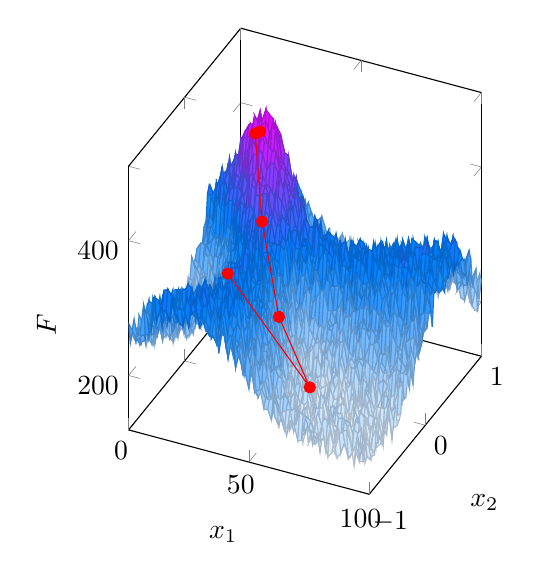
\begin{tikzpicture}
	\begin{axis}[
	width=0.50\textwidth,	
	height = 7.5cm,
	colormap/cool,
	xlabel=$x_1$,
	ylabel=$x_2$,
	zlabel=$F$,
	]
	\addplot3[
	surf,
	%samples = 50,
	domain = 0:100,
	domain y = -1:1,
	]
	{193.0429025 + 137.9330151 *( exp(-(0.05 *(x-25.29101312) + 0.475*sin(deg(0.05 *(x-25.29101312) + 2.5* (y - 0.35586306))))^2) +
		exp(-(2.5* (y - 0.35586306) + 0.475*sin(deg(0.05 *(x-25.29101312) + 2.5 *(y - 0.35586306))))^2)  +
		 (rand-0.5)*2*0.1)
	};
	%{193.043 + 275.866/2 * exp(-(5/100*(x-25.291) + 0.475*sin( 5/100*(x-25.291) + 5/2*(y-0.356))) * exp(-(5/2*(y-0.356) + 0.475*sin( 5/100*(x-25.291) + 5/2*(y-0.356)))};
		\addplot3 [color= red,mark=*,] coordinates {
	(28.125, -0.4375, 320.3734872)
	(65.10367211, -0.562123929, 199.7015173)
	(46.82534862, -0.328866958, 262.9029596)
	(33.05522139, -0.038774837, 361.565507)
	(22.34726992, 0.299065229, 447.3591635)
	(25.01398522, 0.271862773, 455.5853246)
};
	\end{axis}
	\end{tikzpicture}
	\caption{The proposed function $C_4(x_1, x_2)$ for $a = 0.49$.}
	\label{Fig:TwoVarNovelFunc6}
\end{figure}

\begin{figure}
	\centering
	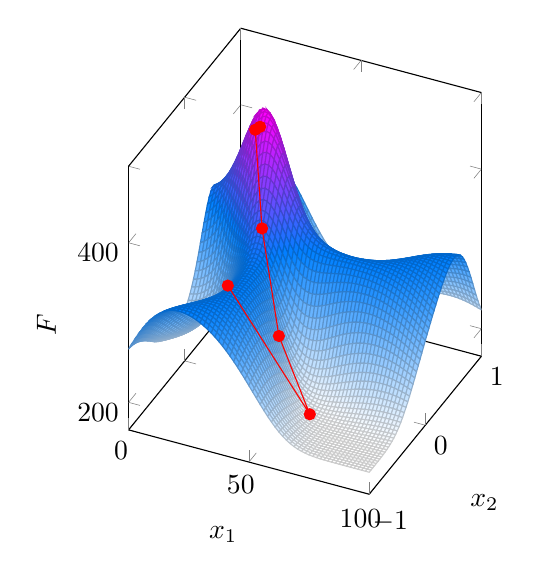
\begin{tikzpicture}
	\begin{axis}[
	width=0.50\textwidth,	
	height = 7.5cm,
	colormap/cool,
	xlabel=$x_1$,
	ylabel=$x_2$,
	zlabel=$F$,
	]
	\addplot3[
	surf,
	%samples = 50,
	domain = 0:100,
	domain y = -1:1,
	]
	{193.0429025 + 137.9330151 *( exp(-(0.05 *(x-25.29101312) + 0.475*sin(deg(0.05 *(x-25.29101312) + 2.5* (y - 0.35586306))))^2) +
		exp(-(2.5* (y - 0.35586306) + 0.475*sin(deg(0.05 *(x-25.29101312) + 2.5 *(y - 0.35586306))))^2)
	};
	%{193.043 + 275.866/2 * exp(-(5/100*(x-25.291) + 0.475*sin( 5/100*(x-25.291) + 5/2*(y-0.356))) * exp(-(5/2*(y-0.356) + 0.475*sin( 5/100*(x-25.291) + 5/2*(y-0.356)))};
	\addplot3 [color= red,mark=*,] coordinates {
		(28.125, -0.4375, 320.3734872)
		(65.10367211, -0.562123929, 199.7015173)
		(46.82534862, -0.328866958, 262.9029596)
		(33.05522139, -0.038774837, 361.565507)
		(22.34726992, 0.299065229, 447.3591635)
		(25.01398522, 0.271862773, 455.5853246)
	};
	\end{axis}
	\end{tikzpicture}
	\caption{The proposed function $C_4(x_1, x_2)$ for $a = 0.49$.}
	\label{Fig:TwoVarNovelFunc4}
\end{figure}

\begin{figure}
	\centering
	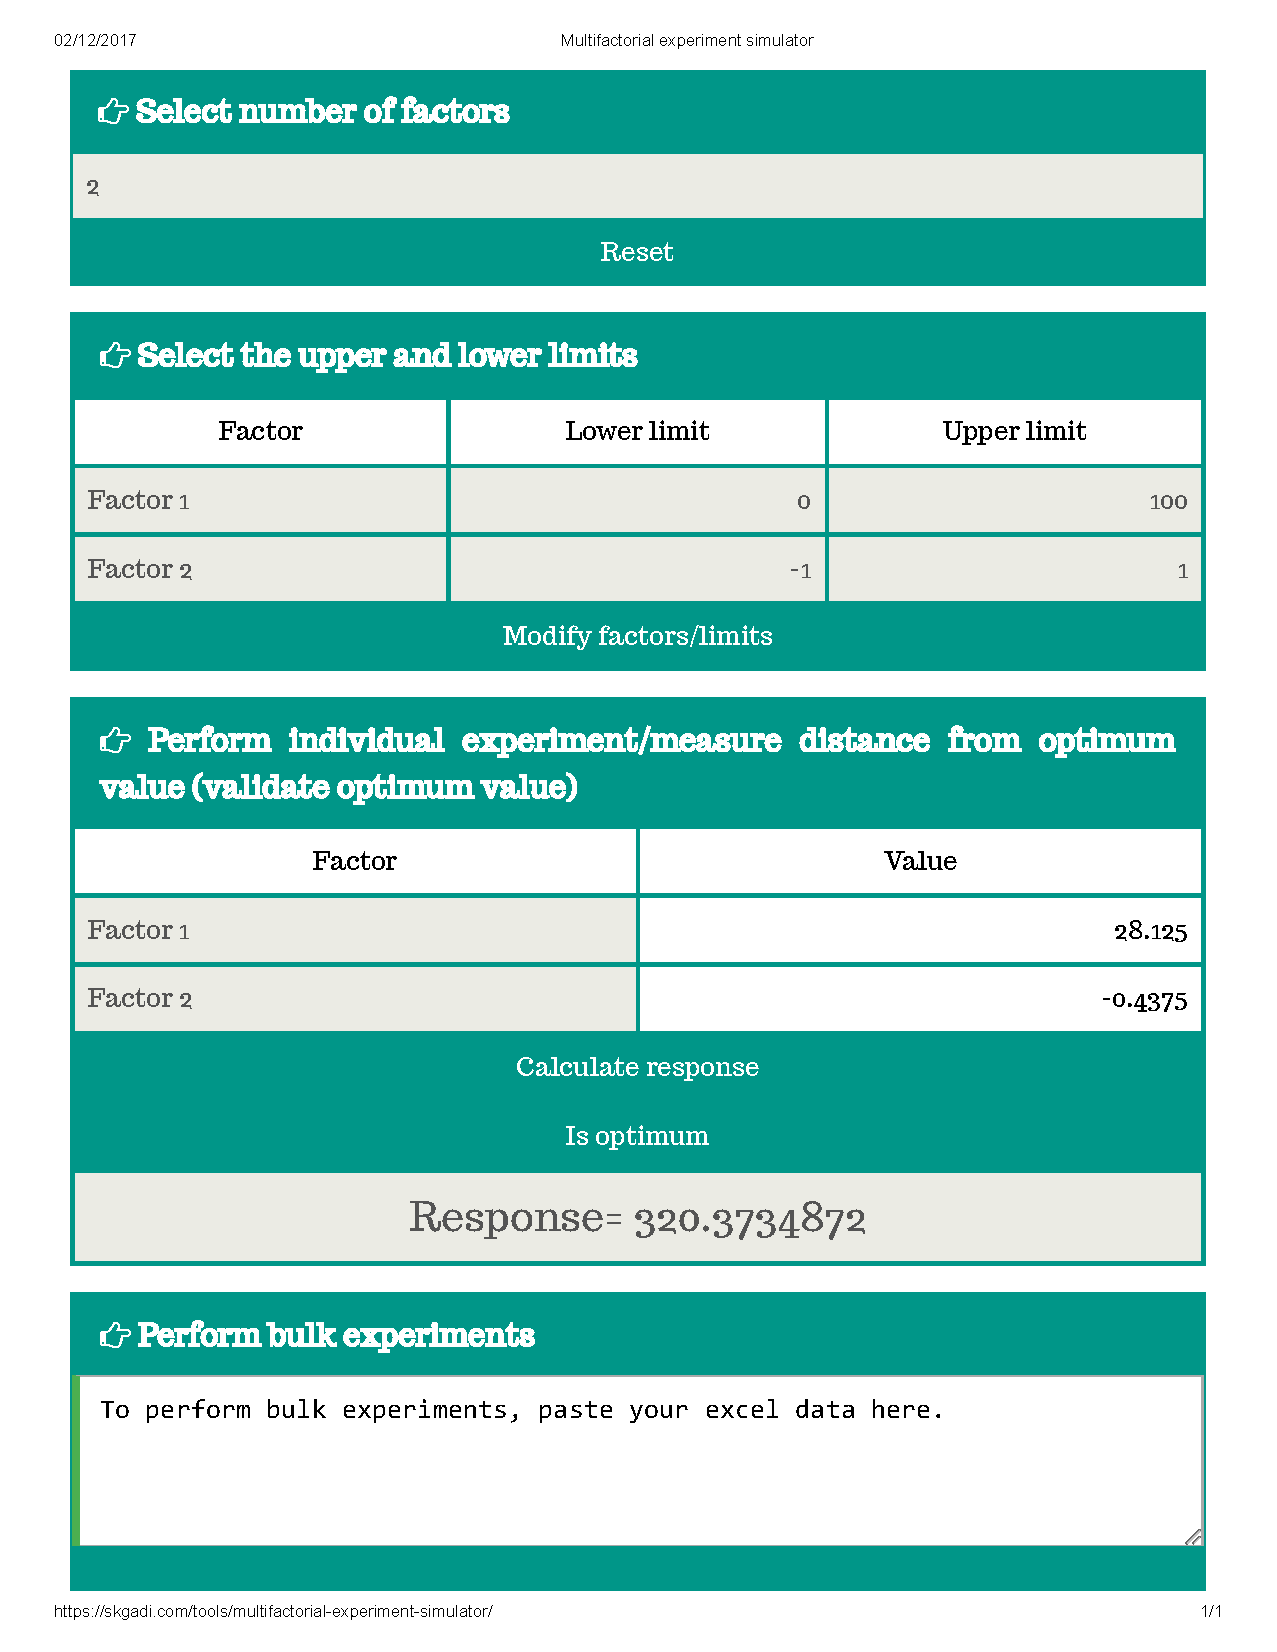
\includegraphics[width=\textwidth]{Ver004-figure9}
	\caption{The proposed function $C_4(x_1, x_2)$ for $a = 0.49$.}
\label{Fig:TwoVarNovelFunc5}
\end{figure}

%\bibliographystyle{apacite}%unsrtnat}
%\bibliographystyle{spbasic}      % basic style, author-year citations
%\bibliographystyle{spmpsci}      % mathematics and physical sciences
%\bibliographystyle{spphys}       % APS-like style for physics
%\bibliographystyle{ieeetr}
%\bibliography{refs}
\end{document}